%% LyX 2.1.4 created this file.  For more info, see http://www.lyx.org/.
%% Do not edit unless you really know what you are doing.
\documentclass[11pt,czech,american]{book}
\usepackage[T1]{fontenc}
\usepackage[utf8]{inputenc}
\usepackage[a4paper]{geometry}
\geometry{verbose,tmargin=4cm,bmargin=3cm,lmargin=3cm,rmargin=2cm,headheight=0.8cm,headsep=1cm,footskip=0.5cm}
\pagestyle{headings}
\setcounter{secnumdepth}{3}
\usepackage{url}
\usepackage{amsmath}
\usepackage{mathtools}
\usepackage{amsthm}
\usepackage{amssymb}
\usepackage{amstext}
\usepackage{graphicx}
\usepackage{setspace}
\usepackage{wrapfig}
\usepackage{algorithm}
\usepackage{algpseudocode}
\usepackage{svg}
\usepackage{outlines}
\usepackage[normalem]{ulem}
\usepackage{dirtytalk}
% \usepackage{subcaption}
% \usepackage{subfigure}

\makeatletter
\newenvironment{lyxlist}[1]
{\begin{list}{}
{\settowidth{\labelwidth}{#1}
 \setlength{\leftmargin}{\labelwidth}
 \addtolength{\leftmargin}{\labelsep}
 \renewcommand{\makelabel}[1]{##1\hfil}}}
{\end{list}}

\usepackage[varg]{txfonts}

\usepackage{indentfirst}

\clubpenalty=9500

\widowpenalty=9500

\hyphenation{CDFA HARDI HiPPIES IKEM InterTrack MEGIDDO MIMD MPFA DICOM ASCLEPIOS MedInria}

\renewcommand{\vec}[1]{\boldsymbol{#1}}
\newcommand{\code}{\texttt}

\newtheorem{thm}{Theorem} % [section]
\newtheorem{lem}{Lemma}
\newtheorem{prop}{Proposition}
\newtheorem{cor}{Corollary}
\newtheorem{conj}{Conjecture}
\newtheorem{dfn}{Definition}

\DeclareMathOperator{\id}{id}
\DeclareMathOperator*{\argmax}{arg\,max}
\DeclareMathOperator*{\argmin}{arg\,min}

% \DeclarePairedDelimiter\ceil{\lceil}{\rceil}
% \DeclarePairedDelimiter\floor{\lfloor}{\rfloor}

\def\code#1{\texttt{#1}}

\newcommand{\bd}[1]{\mathbf{#1}}
\newcommand{\RR}{\mathbb{R}}      
\newcommand{\ZZ}{\mathbb{Z}}
\newcommand{\ZZP}{\mathbb{Z}+^}
\newcommand{\NN}{\mathbb{N}}
\newcommand{\QQ}{\mathbb{Q}}
\newcommand{\CC}{\mathbb{C}}
\newcommand{\col}[1]{\left[\begin{matrix} #1 \end{matrix} \right]}
\newcommand{\comb}[2]{\binom{#1^2 + #2^2}{#1+#2}}
\newcommand{\Tau}{\mathrm{T}}

\DeclarePairedDelimiter\norm{\lVert}{\rVert}

\makeatother

\usepackage{babel}
\begin{document}

\def\documentdate{\today}

\pagestyle{empty}


\noindent \begin{center}
\begin{minipage}[c]{3cm}%
\noindent \begin{center}
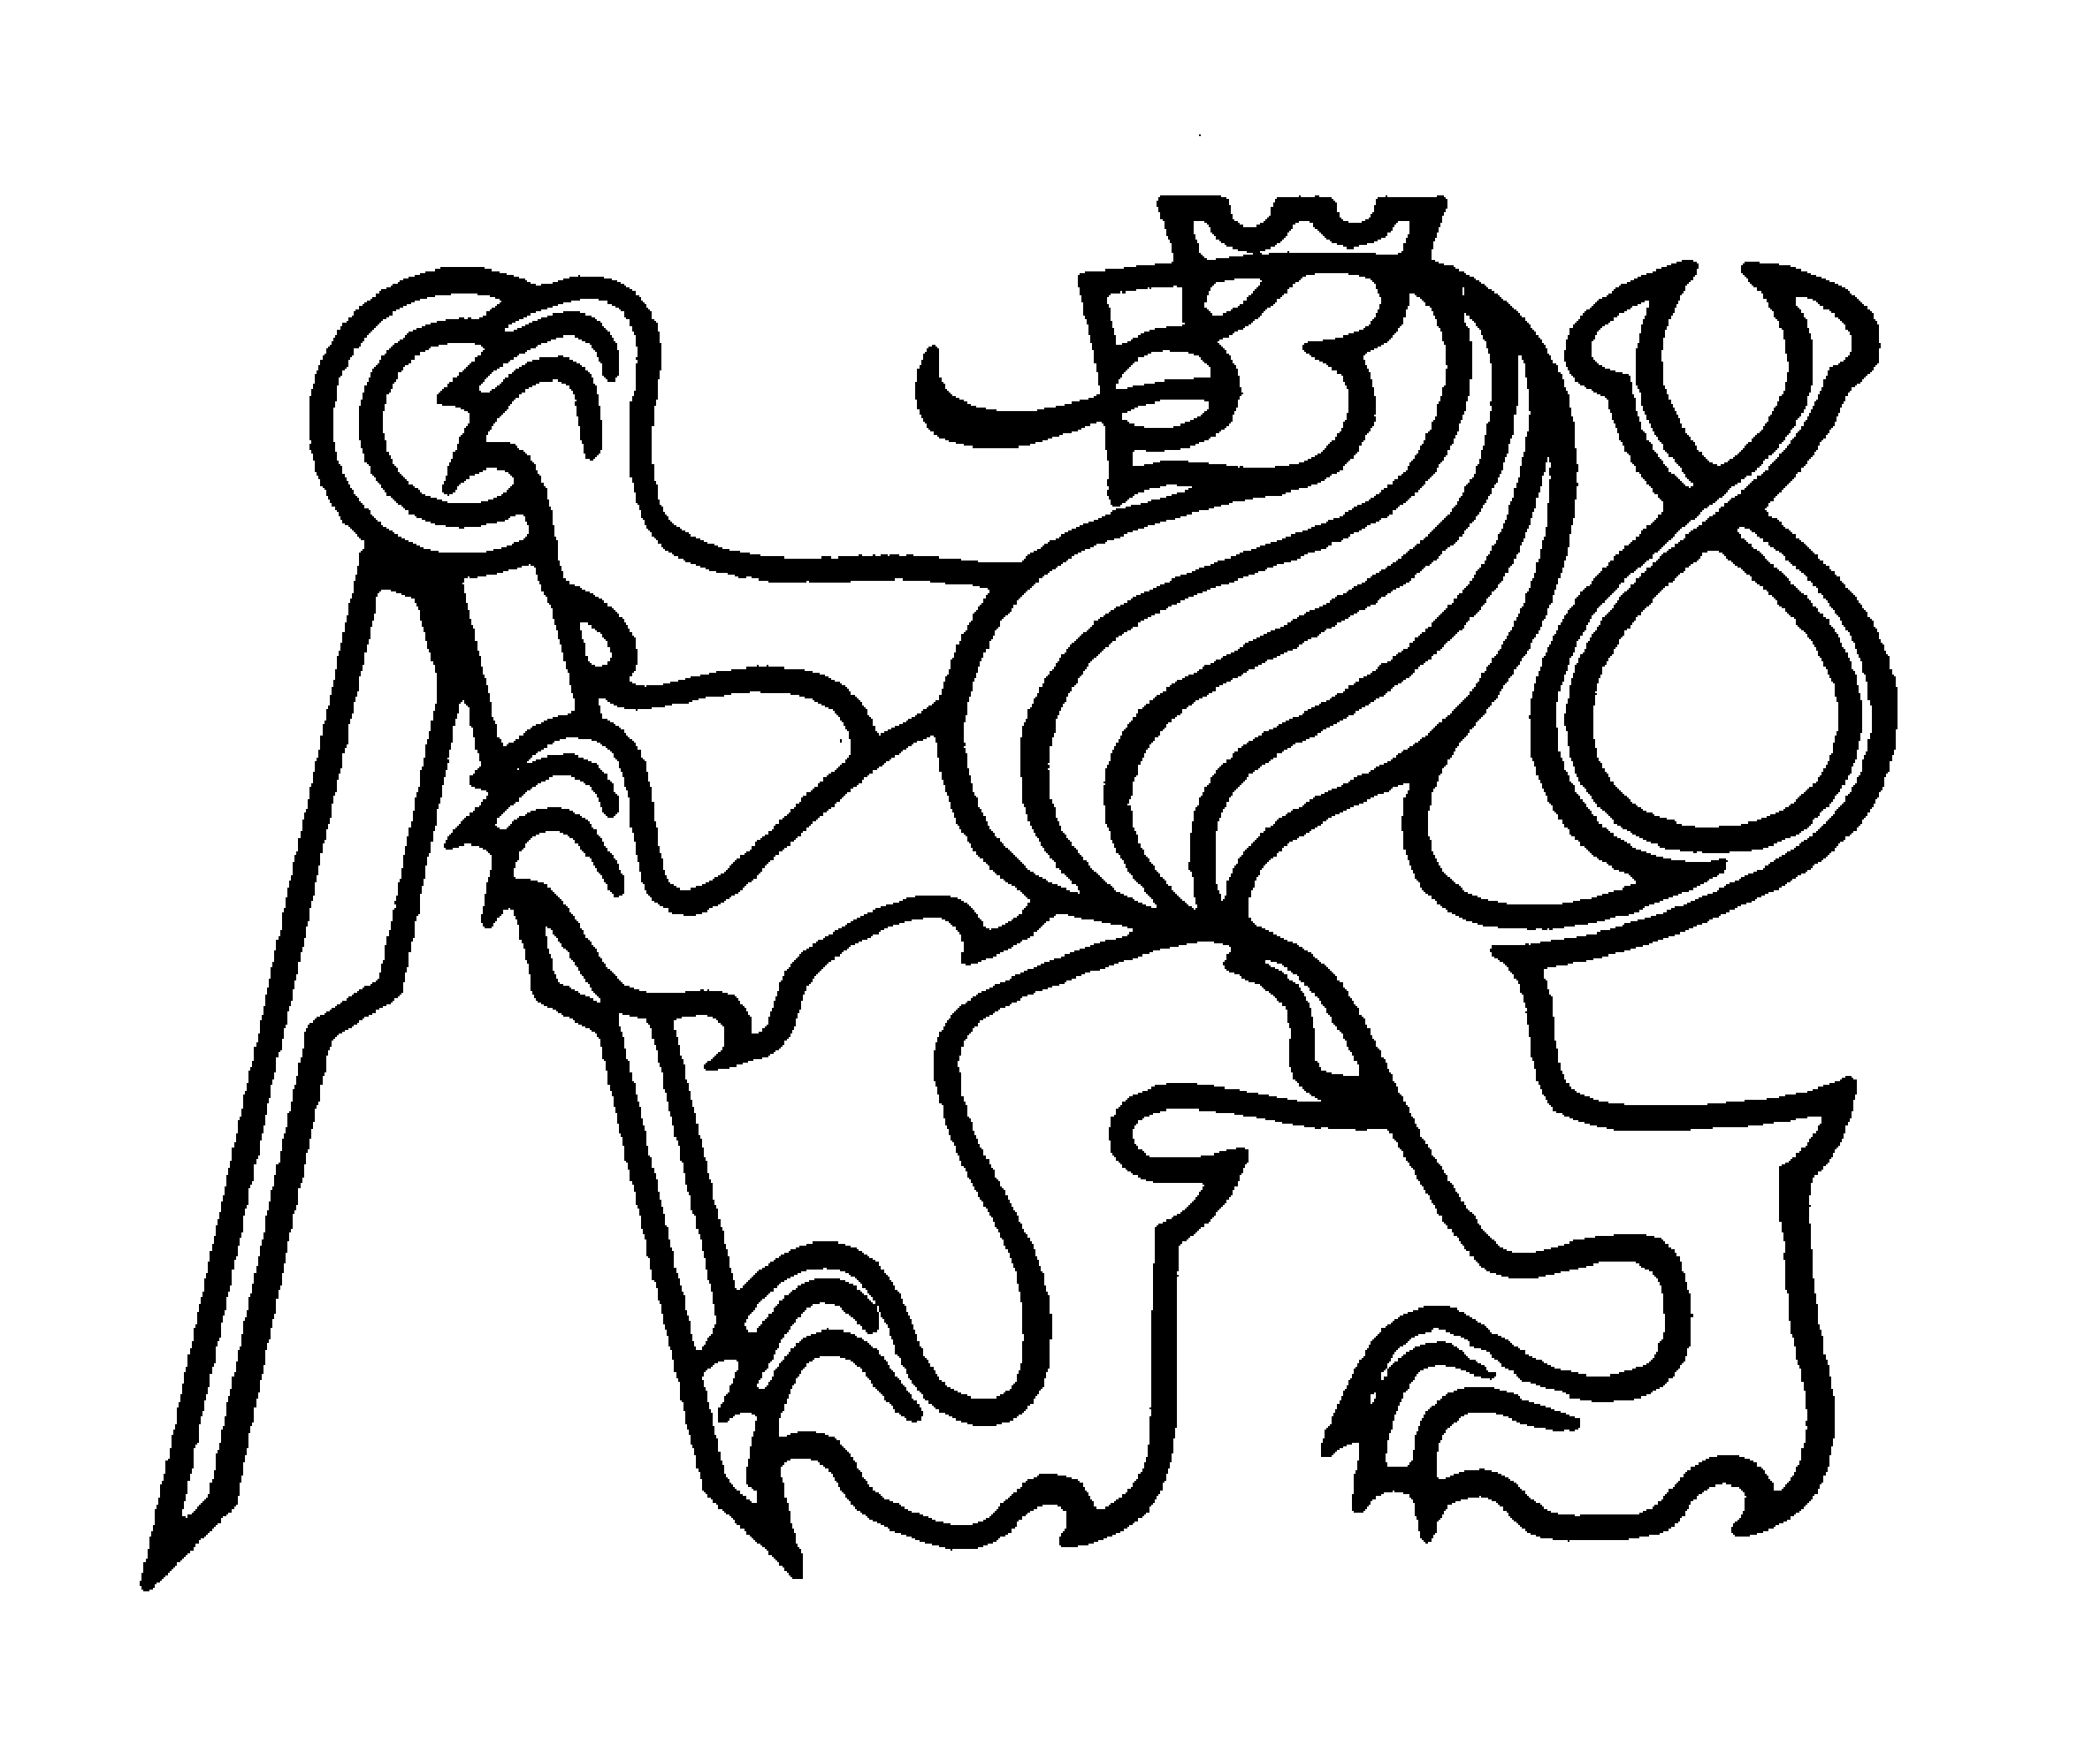
\includegraphics[width=3cm,height=3cm,keepaspectratio]{Images/TITLE/cvut}
\par\end{center}%
\end{minipage}%
\begin{minipage}[c]{0.6\linewidth}%
\begin{center}
\textsc{\large{}Czech Technical University in Prague}{\large{}}\\
{\large{}Faculty of Nuclear Sciences and Physical Engineering}
\par\end{center}%
\end{minipage}%
\begin{minipage}[c]{3cm}%
\noindent \begin{center}

\includegraphics[width=3cm,height=3cm,keepaspectratio]{Images/TITLE/fjfi}
\par\end{center}%
\end{minipage}
\par\end{center}

\vspace{3cm}


\begin{center}
\textbf{\huge{}English Title}
\par\end{center}{\huge \par}

\vspace{1cm}


\selectlanguage{czech}%
\begin{center}
\textbf{\huge{}Czech Title}
\par\end{center}{\huge \par}

\selectlanguage{american}%
\vspace{2cm}


\begin{center}
{\large{}Diploma thesis}
\par\end{center}{\large \par}

\vfill{}

\begin{lyxlist}{MMMMMMMMM}
\begin{singlespace}
\item [{Author:}] \textbf{Miroslav Kovář}
\item [{Supervisor:}] \textbf{M.Sc. M.A. Sebastián Basterrech, Ph.D.}
\end{singlespace}

% \item [{Language~advisor:}] \textbf{Mgr. Jméno Učitelky Angličtiny}
\begin{singlespace}
\item [{Academic~year:}]2018/2019\end{singlespace}

\end{lyxlist}
\newpage{}

~\newpage{}

~

\vfill{}


\begin{center}
- Zadání práce -
\par\end{center}

\vfill{}


~\newpage{}

~

\vfill{}


\begin{center}
- Zadání práce (zadní strana) -
\par\end{center}

\vfill{}


~\newpage{}

\noindent \emph{\Large{}Acknowledgment:}{\Large \par}

\noindent Some acknoledgment here.

\vfill

\noindent \emph{\Large{}Author's declaration:}{\Large \par}

\noindent I declare that this research project is entirely
my own work and I have listed all the used sources in the bibliography.

\bigskip{}


\noindent Prague, \documentdate\hfill{}Miroslav Kovář

\vspace{2cm}


\newpage{}

~\newpage{}

\selectlanguage{czech}%
\begin{onehalfspace}
\noindent \emph{Název práce:}

\noindent \textbf{Czech Title}
\end{onehalfspace}

\bigskip{}


\noindent \emph{Autor:} Miroslav Kovář

\bigskip{}


\noindent \emph{Obor:} Aplikace přírodních věd \bigskip{}


\noindent \emph{Zaměření:} Matematická informatika

\bigskip{}


\noindent \emph{Druh práce:} Diplomová práce

\bigskip{}


\noindent \emph{Vedoucí práce:} M.Sc. M.A. Sebastián Basterrech, Ph.D.,
Artificial Intelligence Center, FEE, CTU Prague

\bigskip{}


% \noindent \emph{Konzultant:} doc. RNDr. Jméno Konzultanta, CSc., pracoviště
% konzultanta. Pouze pokud konzultant byl jmenován.

\bigskip{}


\noindent \emph{Abstrakt:} \bigskip{}


\noindent \emph{Klíčová slova:} 

\selectlanguage{american}%
\vfill{}
~

\begin{onehalfspace}
\noindent \emph{Title:}

\noindent \textbf{English Title}
\end{onehalfspace}

\bigskip{}


\noindent \emph{Author:} Miroslav Kovář

\bigskip{}


\noindent \emph{Abstract:} 

\bigskip{}


\noindent \emph{Key words:} 

%keywords in alphabetical order separated by commas

\newpage{}

~\newpage{}

\pagestyle{plain}

\tableofcontents{}

\newpage{}


\chapter*{Introduction}

% \addcontentsline{toc}{chapter}{Introduction}


\chapter{Classical EEG signal analysis methods}

\section{EEG signal}
Nature, processes in the brain, way of measuring, limitations, complications

Electroencephalography (EEG) is a noninvasive method of measuring fluctuations of electric potentials near the skull caused by synchronized firing of neurons in the upper cortical layers. Electroencephalogram is a record of these fluctuations measured over a period of time. \cite{nunez2006}

Although EEG has significantly lower spatial resolution in comparison with other diagnostic techniques such as functional magnetic resonance sampling (fMRI) and magnetoencephalography (MEG) \cite{srinivasan1999} and enables measuring only neural activity near the cortical surface, as a depression diagnostic tool, it has numerous benefits. Importantly, its significantly lower costs \cite{vespa1999} \cite{hamalainen1993}, high portability, and ease of operation imply increased availability to the patients \cite{schultz2012}. Moreover, it is perfectly noninvasive, which means less complications such as claustrophopia or anxiety \cite{murphy1997}.

Although the science of EEG signal analysis as a diagnostic tool brings compelling clinical promise as a result of the aforementioned benefits, it also presents multiple technical and conceptual challenges. 

\begin{figure} 
\centering
\noindent\makebox[\textwidth]{%
  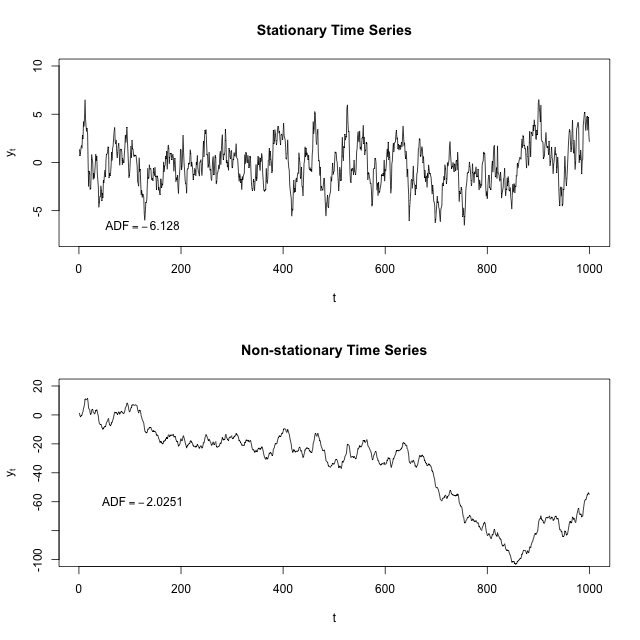
\includegraphics[width=0.8\textwidth]{Images/stationarycomparison.png} }
  \caption{A comparison of stationary and non-stationary time series. (Courtesy: Protonk)}
\label{fig:statnonstatcomp}

\end{figure}
\begin{dfn}[\cite{priestley1988}]
  A series $\{X_t\}_{t \in \ZZ}$ is called \textbf{stationary}, if $\{X_t\}_{t \in \ZZ}$ for any set of times $t_1, t_2, \dots, t_n$ and any $k \in \mathrm{N}$, $P[X_{t_1}, X_{t_2}, \dots, X_{t_n}] = P[X_{t_1+k}, X_{t_2+k}, \dots, X_{t_n+k}]$, i.e. the joint probability distribution of $\{X_t\}_{t \in \ZZ}$ is not a function of time. It is called \textbf{non-stationary}, if it is not stationary.
\end{dfn}

\begin{dfn}[\cite{bickel1996}]
   A series $\{X_t\}_{t \in \ZZ}$ is called (noisy chaotic) \textbf{non-linear}, if it satisfies the relation
   \begin{align}
     X_t = f(X_{t-1}) + \epsilon_t
   \end{align}
   for a general $f : \RR \rightarrow \RR$.
\end{dfn}

EEG signals are prone to be infected with \emph{noise} due to imperfect isolation from surrounding environment. They are known to be \emph{transient, non-Gaussian, non-stationary and nonlinear} \cite{kaplan2005} \cite{stam2005}. Since some patterns do not activate relative to a stimulus, a successful classifier must be able to detect a pattern \emph{regardless of its starting time}, or find one. And finally, EEG records are relatively high dimensional - 16 electrodes sampling at 256 Hz result 4096 data points par second.

Moreover, due to the phenomenon of neural oscillations, patterns may appear in multiple frequency bands, from slow cortical potentials of $\delta$-waves at 0.5-4 Hz, to high $\gamma$ frequency band at 70-150 Hz. 

Patterns of oscillatory activity in various frequency band have been linked to various mental states \cite{canolty2006} \cite{buzsaki2004} and diseases such as epilepsy \cite{shusterman2008}, tremor \cite{mcauley2000}, Parkinson's disease and depression \cite{llinas1999}. Many of the diseases, including depression, share common oscillatory patterns known as thalamocortical dysrythmia, characterized by descrease in normal resting-state $\alpha$ (8-12 Hz) activity slowing down to $\theta$ (4-8 Hz) frequencies, accompanied by increase in $\beta$ and $\gamma$ (25-50 Hz) activity. \cite{vanneste2018}

\section{Non-linear time series analysis}
Modern neuroscientific work suggests that the most plausible research target for explaining the brain dynamics are the assemblies of coupled and synchronously active neurons, and since majority of those assemblies are describable by non-linear differential equations, it is common to apply principles derived from nonlinear dynamics to characterize these neuronal systems.\cite{kaplan2005} In this section, we will describe some of those principles.

Attractors, Poincare plots, recurrence plots, Lyapunov coefficients, fractal dimension, Hurst exponent, etc.

\begin{dfn}[\cite{kantz2004}]
  Let $\mathbf{x} \in \RR^m$ be an $m \in NN$ dimensional state space vector dependent on time. A deterministic \textbf{dynamical system} is described by a set of $m$ first-order differential equations
  \begin{align}
    \frac{d}{dt}\mathbf{x}(t) = \mathbf{f}(\mathbf{x}(t)), \qquad t \in \RR
  \end{align}
\end{dfn}

In other words, a dynamical system is a model that determines the evolution of a system only given by the initial state, and current state is a function of the previous state. Hence, a total description of a dynamical system is given by the initial state and a set of equations. A non-linear dynamical system is a system where the differential equations describing its dynamics are non-linear. Unlike in a linear system, changes in the initial state of a non-dynamical system are allowed to have a non-linear relationship to the state space trajectory of the system. \cite{kaplan2005}

\subsection{Attractor}
\begin{dfn}[\cite{kantz2004}]
  A dynamical system is called dissipative, when it is the case that
  \begin{align}
    E[\mathrm{div} \mathbf{f}] < 1
  \end{align}
\end{dfn}

In other words, average space space volume (containing the initial state) is contracted as the system evolves.

Dissipative dynamical system have the property that a set of initial states (of positive measure) will converge to a subspace of the overall state space. This subspace is a geometrical object called an \textbf{attractor}. Example of four basic attractors can be seen on Figure \ref{fig:attractors}.

\begin{figure} 
\centering
\noindent\makebox[\textwidth]{%
  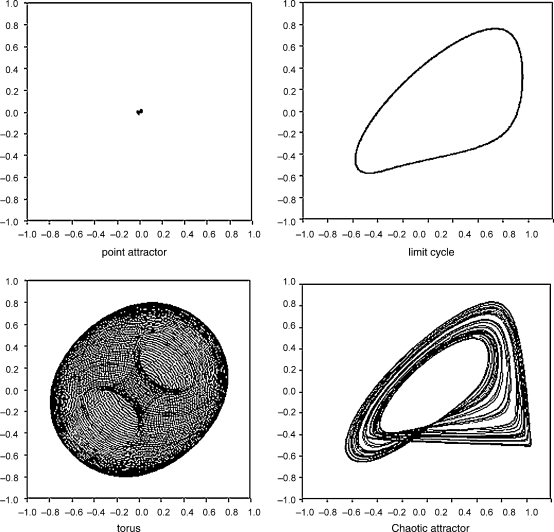
\includegraphics[width=0.8\textwidth]{Images/attractors.png} }
  \caption{Visualization of four common attractor types (units are arbitrary). Left to right, top to bottom:
    \emph{Point attractor} is the only type of attractor of linear deterministic dissipative systems.
    \emph{Limit cycle} corresponds to a peridic system.
    \emph{Torus attractor} corresponds to a quasi-periodic system, resulting (in this example) from a superposition of two periodic oscillations.
    \emph{Chaotic} (strange) \emph{attractor}, characterized by strong dependence on the original conditions. (\cite{stam2005})}
\label{fig:attractors}
\end{figure}

Since most physiogenerated signals are chaotic, their analysis is concerned primarily with \emph{chaotic} (strange) \emph{attractors}. These attractors are complex, and exhibit what is known as \emph{fractal geometry} (an example of a self-similar attractor is shown on Figure \ref{fig:self-similarity}).
. For our purposes, this means they can be characterized as having quantifiable self-similarity.\footnote{Cantor set being a canonical example of self-similarity.} However, the following definition will be useful:

\begin{dfn}[\cite{falconer2004}]
  Let $F$ be any non-empty bounded subset of $\RR^n$, and let $N_\epsilon(F)$ be the smallest number of sets of diameter at most $\epsilon$ which can cover $F$. Then, the \textbf{box-counting dimension} (also known as Minkowski–Bouligand dimension) is defined as
  \begin{align}
    d_F = \lim_{\epsilon \rightarrow 0} \frac{\log N_\epsilon(F)}{\log{\frac{1}{\epsilon}}} \, ,
  \end{align}
  if it exists.
\end{dfn}

Intuitively, the number of mesh cubes of side $\epsilon$ intersecting $F$ gives an indication about how irregular the set is when inspected at scale $\epsilon$, and the box-counting dimension reflects ``how rapidly'' the irregularities develop as $\epsilon \rightarrow 0$. \cite{falconer2004} 

\begin{figure} 
\centering
\noindent\makebox[\textwidth]{%
  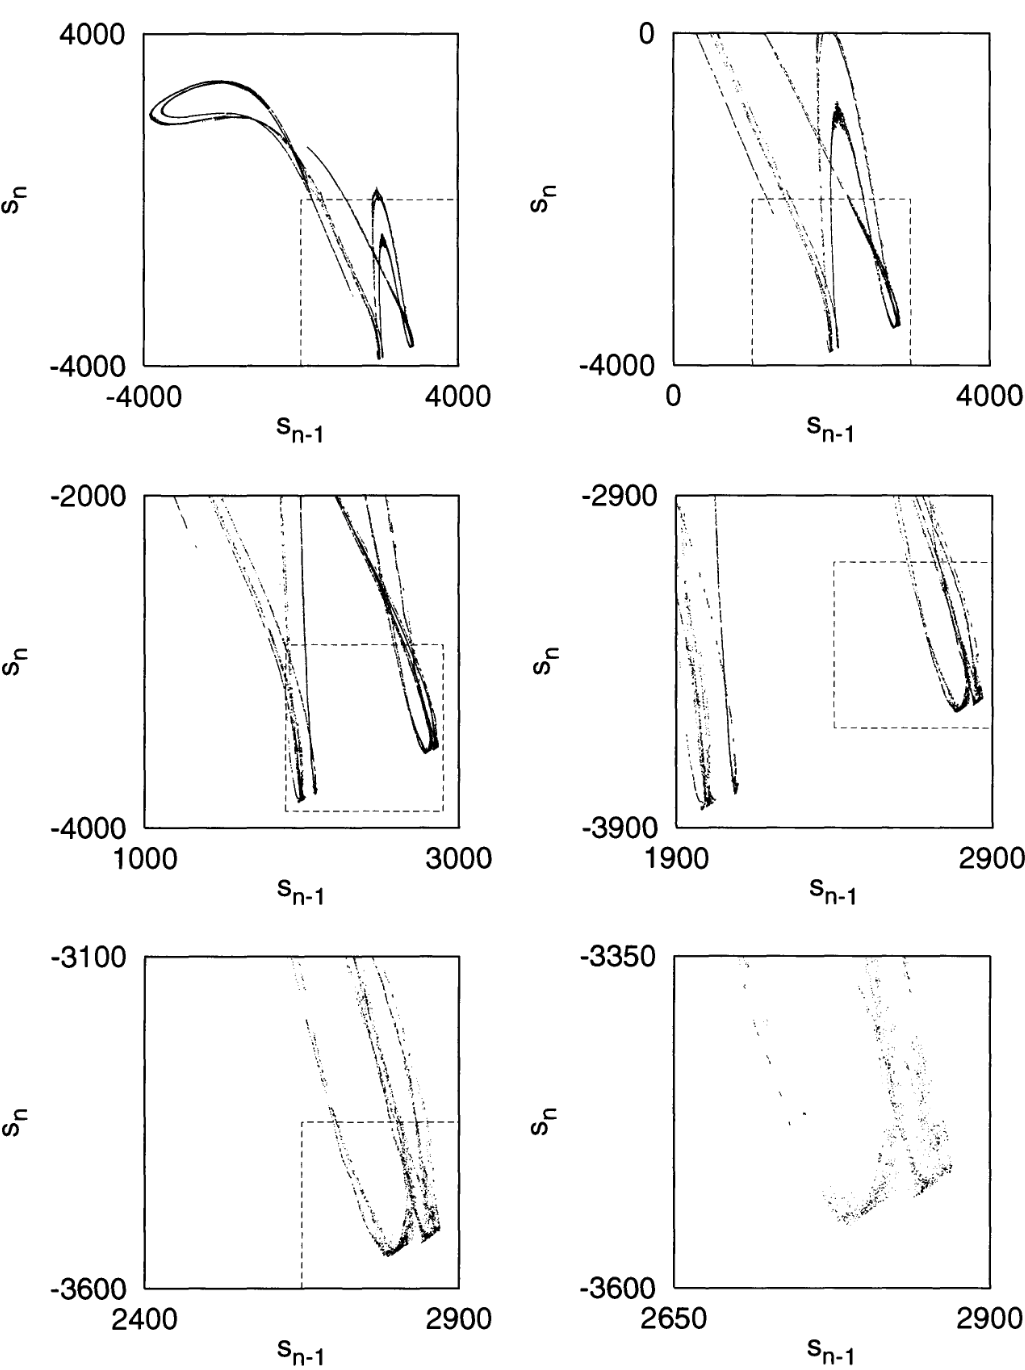
\includegraphics[width=0.8\textwidth]{Images/self-similarity.png}}
  \caption{Noise-reduced visualization of successive enlargements of highly self-similar attractor. (\cite{kantz2004})}
\label{fig:self-similarity}
\end{figure}

\subsection{Embedding}
One possible approach to non-linear time series analysis consists of the following steps: 
\begin{enumerate}
  \item reconstruction of the dynamics of given system from recorded data,
  \item characterization of the reconstructed attractor,
  \item checking validity of the results with surrogate data testing. \cite{stam2005}
\end{enumerate}

In the following text, we will describe multiple techniques of characterizing the properties of attractors (and hence ways of describing the dynamics of the dynamical system) using these steps.

In order to reconstruct the dynamics of given system from recorded data, it is necessary to deal with the fact that our data, however rich, rarely represent complete information about the studied system. In the case of EEG signals, the complete state of the system at any moment is determined by many variables, and the sensors are only able to collect traces of their cumulative effects (and noise). The process known as \emph{state} (phase) \emph{space reconstruction via the method of time delays} is a way of reconstructing the attractor of given dynamical system from single (or multiple) sequences of scalar measurements.

The following result from 1936 was important for theoretical understanding of time delay embeddings:
\begin{thm}[Whitney embedding theorem, \cite{whitney1936}]\label{thm:whitney}
  Every $n$-dimensional differentiable manifold can be embedded in $\RR^{2n}$.
\end{thm}

N. H. Packard has proposed in \cite{packard1980} a process by which a time series of measurements sampled at regular intervals can be embededded into a $n$-dimensional space in such a way that the series of reconstructed vectors is representative of the dynamics of the system. A year later, in \cite{takens1981}, F. Takens has proved theoretically, using Whitney's result, that the reconstructed attractor has the same dynamical properties (entropy, dimension, Lyapunov spectrum) as attractor of the original system.

Takens delay embedding theorem is an important result of non-linear time series analysis and can be stated as follows:
\begin{thm}[\cite{takens1981}] \label{thm:takens}
  Let $M$ be a compact\footnote{This theorem can be proved for $M$ non-compact provided less restrictions are imposed on $s$.} manifold specifying the state space of a deterministic dynamical system of dimension $n \in \NN$, $s : M \rightarrow \RR, s \in C^2$ a smooth measurement function, $f : M \rightarrow M, f \in C^2$ a smooth diffeomorphic state evolution function with a strange attractor of box-counting dimension $d_A$, and let $k > 2d_A$. Then a map $\phi : M \rightarrow \RR^k$, defined by
  \begin{align}
    \phi(x) = (s(\mathbf{x}), s(f(\mathbf{x})), \dots, s(f^{k-1}(\mathbf{x})))
  \end{align}
  is an embedding.
\end{thm}

In what follows, we will describe how these results can be applied in practice. Let us have a time series of scalar measurements of a quantity depending on the current state of the system:
\begin{align}
  s_n = s(\mathbf{x}(n \Delta t)) + \eta_n \, ,
\end{align}
where $\mathbf{x}$ is a state space vector, $s(\cdot)$ is a measurement function and $\eta_n$ is a measurement noise.

Then, the time delay reconstruction is then simply formed by the following vectors:
\begin{align}
  \textbf{s}_n = (s_{n-(m-1)\tau}, s_{n-(m-2)\tau},\dots,s_{n-\tau}, s_n) \, ,
\end{align}

for $n > (m-1)\tau$. \cite{kantz2004} 

Of course, this method requires proper choice of parameters $m$ and $\tau$. From Theorem \ref{thm:takens} follows that vectors $\{\mathbf{s}_n\}$ are difeomorphic to the attractor $A$ of the system $M$ if $m$ is sufficiently large, specifically $m > 2d_A$ (note that $d_A$ may be much smaller than $\dim M$). On the other hand, $m$ adds redundancy, makes successive alogorithms less efficient. Moreover, the total time delay $m\tau$ is limited by the recording time. 

There are multiple methods of choosing the parameters. We will start with a description of an algorithm for determining the minimal sufficient embedding dimension $m$. It uses concept known as \emph{false nearest neighbors}.

(TODO: False nearest neighbors? The problem is I don't know if I need to go deep into this topic because we may simply end up using meta-recurrence plots. We may try computing non linear analysis parameters and train a NN classifier on them and compare (which seems more reasonable than CapsNets). I like the idea.)

(TODO: Mutual information algorithm for $\tau$)

(TODO: Mention spatial embedding. Is it worth using for EEG analysis? Pro: it achieves considerable reduction. Con: we may lose valuable information.)

\subsection{Measures of non-linear interdependency}
Phase synchronization, synchronization measures - we can use them to quantify interactions between brain regions. May be useful.

\subsection{Recurrence plot}
When presented with a task of finding regularities in seemingly chaotic data, one possible approach is analysing at least approximate repetitions of simple patterns, which can be further used for reconstruction of more complicated rules. Recurrence plot is a method of visualizing obtained state-space trajectory segments in relation to each other to achieve this goal. Furthermore, it can be used to test necessary conditions for validity of dynamical parameters derivable from a non-linear time series such as the information dimension, entropy, Lyapunov exponents, dimension spectrum, etc. The information contained in recurrence plots is not easily obtainable by other known methods. \cite{eckmann1987}

\begin{dfn}[\cite{eckmann1987}]
  Let $N$ be the length of given time series, $\mathbf{s}_i$ for $i \in \{1,2,\dots,N \}$ be a $i$-th delay vector of any integer embedding dimension, $\norm{\cdot}$ a norm, $\Theta(\cdot)$ a Heaviside step function, and $\epsilon \in \RR_0^+$ a tolerance parameter. Then, \textbf{recurrence plot} is the matrix
  \begin{align}
    M_{ij} = \Theta(\epsilon - \norm{ \textbf{s}_i - \textbf{s}_j }) \, .
  \end{align}
\end{dfn}

In other words, $M_{ij}$ is a symmetric\footnote{Although this is true for our definition, it may not be true for an alternative definition using a more general topology instead of a norm.} binary $N x N$ matrix, where $M_{ij} = 1$ when $i$-th and $j$-th points of the reconstructed trajectory enter each other's $\epsilon$ neighborhood.

The essential drawback of recurrence plot is their size - it is quadratic in the length of the time series. A simple way of reducing its dimension is to partition the time series into disjoined segments, and let $M_{ij}$ represent the distance between those two segments. This is known as \textbf{meta-recurrence plot}. \cite{kantz2004} (TODO: Find a justification for using them.)

(TODO: Cross-recurrence plots may be useful? Only between two series. Joint recurrence plots may be used to detect phase synchronization.)

\section{Applications}
Results in applying classical methods and deep learning to EEG signal analysis

The number of studies applying methods of non-linear time series analysis for clinical depression diagnosis is limited. Abnormalities in sleep EEG have been found, as well as increased predictablity of waking EEG. \cite{nandrino1994}

\chapter{Convolutional Neural Networks}

\section{Mathematical background}
TODO: Do we really need this section???
Very briefly (everyone knows): fully connected, gradient based learning (backpropagation), invariance.

\begin{dfn}
  Let $I$ be an image function, $K$ a kernel. A (discrete) \textbf{convolution} of $I$ and $K$ is a functional defined as
  \begin{align}
    (I*K)(i,j) = \sum_m \sum_n I(m,n) K(i-m, j-n) \, .
  \end{align}
\end{dfn}

Note that some machine learning libraries (such as Tensorflow) implement \textbf{cross-correlation} instead of convolution, but preserving the term convolution for the operation. Cross-correlation corresponds to convolution with kernel rotated by 90 degrees:
\begin{align}
  (I*K)(i,j) = \sum_m \sum_n I(m,n) K(i+m, j+n) \, .
\end{align}
Unlike convolution, cross-correlation is not commutative, but this property is not required for neural network applications.

For the following, the reader needs to understand the term \textbf{equivariance}. 
\begin{dfn}[\cite{pitts2013}]
  Let $G$ be a group and $X$, $Y$ its G-sets. Then $F:X \rightarrow Y$ is called an \textbf{equivariant function} if
  \begin{align}
    F(g(x)) = g(F(x))
  \end{align}
  for all $G$ actions $g$ and $x \in X$.
\end{dfn}

For our purposes, we can view $G$ as a group of transformations, and then equivariance as a commutative property of a function with regards to the transformations. In other words, computing the function and then applying the transformation has the same effect as applying the transformation and then computing the function.

\section{History}

The classical approach to image pattern recognition consists of the following stages:
\begin{description}
  \item[preprocessing:] supressing unwanted distortions and noise, enhancement beneficient for further processing,
  \item[object segmetation:] separating disparate objects from the background,
  \item[feature extraction:] gathering relevant information about the properties of the objects, removing irrelevant variations,
  \item[classification:] categorizing segmented objects based on obtained features into classes.
\end{description}

The preprocessing step may require additional assumptions about the data or further processing, which are potentially too restrictive or too broad. Getting around this limitation requires dealing with complications such as high dimensionality of the input (number of pixels) and desirability of invariance towards a number of allowable distortions and geometrical transformations.

Artificial neural networks in combination with gradient-based learning are one possible solution to the problem. By gradually optimizing a set of weights based on a training data set using a differentiable error function, they provide a framework for learning a suitable set of assumptions automatically from the data.

One of the oldest neural network architectures, fully connected multi-layer perceptron (FC-MLP), can be used for image pattern recognition. However, it has the following drawbacks:
\begin{description}
  \item[parameter explosion:] the number of parameters of such network is exponential in the number of layers, increasing the capacity of the network and therefore need for more data,
  \item[no invariance:] no invariance even with respect to common geometrical transformation such as translation, rotation and scaling,
  \item[ignoring input topology:] natural images exhibit strong local structure and high correlation between intensities of neighboring pixels, but FC-MLPs are unstructed - inputs can be presented in any order.
\end{description}

Although the main idea dates back 1980 with K. Fukushima's neocognitron \cite{fukushima1982}, the back-propagation algorithm was not known at the time. The first convolutional architecture successfuly applied on an image pattern recognition problem by attempting to solve the aforementioned problems, dubbed LeNet-5, was proposed in 1998 by Y. LeCun, L. Bottou, Y. Bengio and P. Haffner \cite{LeCun1998}.

\section{Description}

\begin{figure} 
\centering
\noindent\makebox[\textwidth]{%
  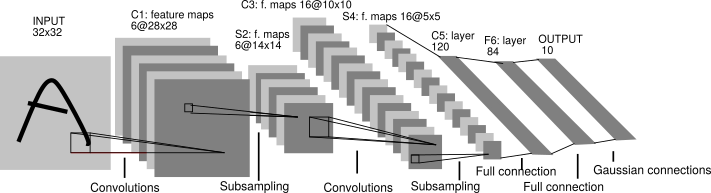
\includegraphics[width=0.8\textwidth]{Images/lenet-5.png} }
  \caption{LeNet-5 architecture \cite{lecun1999}.}
\label{fig:lenet-5}
\end{figure}

Bearing resemblence to visual processing in biological organisms \footnote{As early as in 1968, D. H. Hubel and T.N. Wiesel discovered that some cells (called simple cells) in cat's primary visual cortex (V1) with small receptive fields (shared by neighboring neurons) are sensitive to straight lines and edges of light of particular orientation, and other cells (called complex cells) with larger receptive fields further in the visual cortex also respond to straight lines and edges, but with invariance to translation \cite{Hubel1968}.}, LeNet-5 proposed the following design principles to enforce \emph{shift, scale and distortion invariance}: \cite{lecun1999}
\begin{description}
  \item[local receptive fields:] each neuron in a layer receives input from a small neighborhood in the previous layer,
  \item[shared weights:] each layer is composed of neurons organized in planes within which each neuron have the same weight vector (feature map),
  \item[spatial subsampling:] adding a subsampling layers, which reduce the resolution of the previous layer by averaging or taking the maximal value of neighboring pixels in the previous layer.
\end{description}

\subsection{Local receptive fields}
\emph{Local receptive fields} enable the network to synthesize filters that produce strong response to elementary salient features in the early layers (such as lines, edges and corners in a visual input, and their equivalents in other modalities), and then learn to combine them in the subsequent layers to produce higher-order feature detectors.

\begin{figure} 
\centering
\noindent\makebox[\textwidth]{%
  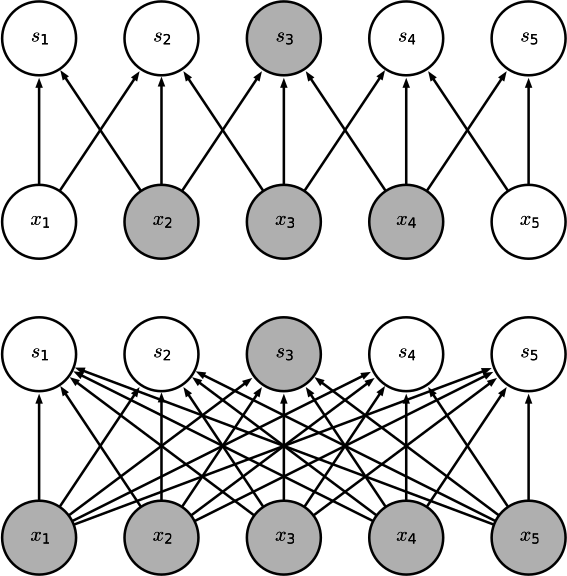
\includegraphics[width=0.5\textwidth]{Images/receptive_field.png} }
  \caption{Receptive field. \cite{goodfellow2016}}
\label{fig:receptive_field}
\end{figure}

For a visual explanation of the concept of receptive field, see Figure \ref{fig:receptive_field}. The locality of of those receptive fields implies sparser connectivity, and hence more efficient computations in comparison with fully connected neural networks. A fully connected neural network with no hidden layers with $m$ inputs and $n$ outputs has $m \times n$ weight parameters, and the correspoding feed forward pass (matrix multiplication) is of $O(m \times n)$ time complexity per input. If the number of connections per output unit is limited to $k < m$, the achieved runtime is $O(k \times n)$, where $k$ is usally in practice several orders of magintude smaller than $m$. \cite{goodfellow2016}

In shallow neural networks, locality of receptive fields implies locality of ``influence'' of each input unit on the output. In deep neural networks, on the other hand, units in the deeper layers can be indirectly connected to some or all units of the input, thus enabling them to achieve aforementioned effect of combining more complex features from simpler ones.

\subsection{Shared weights}
With \emph{shared weights}, neural units in a layer with differing receptive fields have the same feature map and the same feature detecting operation (convolution with feature map kernel followed by additive bias and a application of a non-linear function) is performed on differing parts of the image (see Figure \ref{fig:shared_weights}). A single convolutional layer is composed of multiple feature detecting planes.

Shared weights principle exploits the fact that in natural images, a function of small number of neighboring pixels can be useful in multiple parts of the image. For example, an edge detector can be used accross the entire image to detect edges in the first layer, an object detector can then be used to detect presence of edges in particular arrangements in the next layer, etc.

Although it does not reduce the time complexity of the feedforward pass, it does reduce the memory requirements. If the kernel size is $k$, $m$ the number of inputs, $n$ the number of outputs, the number of parameters per layer is $k$ instead of $m \times n$ (per feature detecting plane) in a fully connected case. Since $k$ is usually in practice several orders of magnitude smaller than $m$, and usually $m$ and $n$ are comparable in size, the memory savings are highly significant. \cite{goodfellow2016}

One of the drawbacks of classical CNNs is that although convolution in combination with weight sharing causes layer output to be equivariant to translation of the input, this is not the case for scaling and rotation. Moreover, equivariance to input may not be always desirable. Consider a case of face detection, where all training and test images are centered. Then, the relative positions of individual features are important, and it may be favorable to fix feature detectors (and thus weights) to certain locations in the image.

\subsection{Pooling}
\begin{figure} 
\centering
\noindent\makebox[\textwidth]{%
  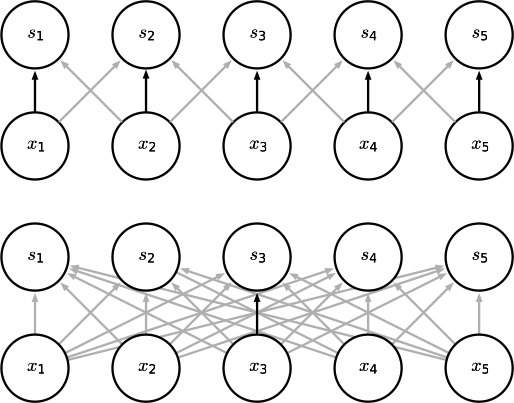
\includegraphics[width=0.5\textwidth]{Images/shared_weights.png} }
  \caption{Shared weights. \cite{goodfellow2016}}
\label{fig:shared_weights}
\end{figure}

The final output activations of a convolutional layer are computed in subsequent stages:
\begin{enumerate}
  \item linear unit activations are computed via the convolution operation,
  \item a non-linear activation function is applied to the activations,
  \item a spatial subsampling (pooling) operation is applied.
\end{enumerate}

One of the main reasons for applying a non-linearity is to make the network capable of modelling non-linear functions. Common activation functions include rectified linear $\max(0,x)$, sigmoid $\frac{1}{1+\exp(-x)}$, hyperbolic tangent $\tanh$, and many others. They have varying properties making them useful in different situations. We will not explore them further here.

\emph{Pooling} operation splits the neural units into disjoint sets of multiple adjacent activations and computes a summary statistic per such set and outputs the result. Thus the spatial dimension of output is decreased relative to input (subsampling).

The purpose of spatial subsampling is to ensure scale and distortion invariance\footnote{Whether it achieves this goal has been famously doubted by Geoffrey Hinton: ``The pooling operation used in convolutional neural networks is a big mistake and the fact that it works so well is a disaster.'' \cite{}} by reducing the precision at which a feature is encoded in a feature map by reducing its resolution - when scale and distortion invariance is assumed, the exact location of a feature becomes less important and is allowed to exhibit slight positional variance - roughly speaking, an ``approximate'' translation invariance. Although this simple solution performs well in many practical situations, it has multiple drawbacks. 

TODO: relative representation of features is not encoded in the feature map representation.

\section{Applications}
Maybe mention an example of how LeNet-5 was improved on subsequently (AlexNet, ResNet, etc.)? But this changes all the time\dots

\section{CapsNets?} \label{sec:capsnets}
Does it make sense trying them? I found a only a few successful implementations. Maybe it would be better to try those after we have some results already, because it seems risky - we might end up with nothing.

\chapter{Experiments}

\section{Dataset}
Size of our dataset, conditions during trials, labels, etc.

\section{Results}


\chapter*{Conclusion}


\bibliographystyle{plain}
\bibliography{refs}
\end{document}
